% -------------------------------------------------
\section{Ledger Dynamics \& Born Rule}
\label{sec:born}
% -------------------------------------------------

With the number tower in place (Section~\ref{sec:number}) we now translate
ledger counting into \emph{physical dynamics}.  The central result of this
section is that the Born probability rule drops out as an \emph{identity},
not a postulate.

\subsection{Branch amplitude recurrence}

Recall the quarter-turn update fixed by the Uniqueness Theorem
(Section~\ref{sec:axioms}):

\[
  \Psi_{n+1}(s\pm)=\frac{1}{\sqrt2}\,
  e^{\pm i\pi/2}\,\Psi_n(s), \qquad
  s\in\{+,-\}^{n}.
\tag{4.1}\label{eq:quarter-turn}
\]

Iterating Eq.~\eqref{eq:quarter-turn} over $n$ steps yields

\[
  \Psi_n(s)=2^{-n/2}\exp\!\Bigl(
    \tfrac{\pi i}{2}\,[\#(+)-\#(-)]
  \Bigr),
\tag{4.2}\label{eq:amplitude-form}
\]

where $\#(\pm)$ counts the occurrences of $+$ or $-$ in the tag string
$s$.  The ledger thus \emph{stores} both modulus and phase as branch
counters; no external Hilbert space is needed.

\subsection{Weight conservation implies Born rule}

Define the \emph{weight} of a tag set $S\subset\{+,-\}^n$ as

\[
  W_n(S):=\sum_{s\in S} \lvert\Psi_n(s)\rvert^{2}.
\]

Using Eq.~\eqref{eq:amplitude-form} the modulus is $2^{-n}$ for every
branch, so

\[
  W_n(S)=2^{-n}\,\#(S).
\tag{4.3}\label{eq:weight-count}
\]

If $S$ and $T$ are disjoint tag sets representing two outcomes of an
experiment, then

\[
  \frac{W_n(S)}{W_n(S)+W_n(T)}
  =\frac{\#(S)}{\#(S)+\#(T)},
\tag{4.4}\label{eq:born}
\]

\emph{exactly} the Born rule: probability equals branch-number ratio.

\begin{theorem}[Born rule is a counting identity]
Under Axioms 1–2 and the recursion
Eq.~\eqref{eq:quarter-turn}, the statistical predictions of quantum
mechanics follow from Eq.~\eqref{eq:born} without additional postulates.
\end{theorem}

\begin{proof}
Ledger weight is conserved by construction.  Equation~\eqref{eq:weight-count}
relates weight to branch count, and Eq.~\eqref{eq:born} is then merely the
definition of relative frequency.  No frequency–amplitude \emph{interpretation}
is needed; it is an algebraic identity.
\end{proof}

\subsection{Interference as ledger phase cancellation}

Consider two depth-$n$ branches whose tag difference is a single bit
flip.  Their phase difference by Eq.~\eqref{eq:amplitude-form} is
$\pi$, so they \emph{destructively interfere}.
Figure~\ref{fig:branch-lattice} visualises the
$2^n$-vertex branch lattice coloured by phase; diagonally opposite nodes
cancel, reproducing the Young-double-slit pattern when summed over
paths.

\begin{figure}[t]
  \centering
  \setkeys{Gin}{draft=false}%
  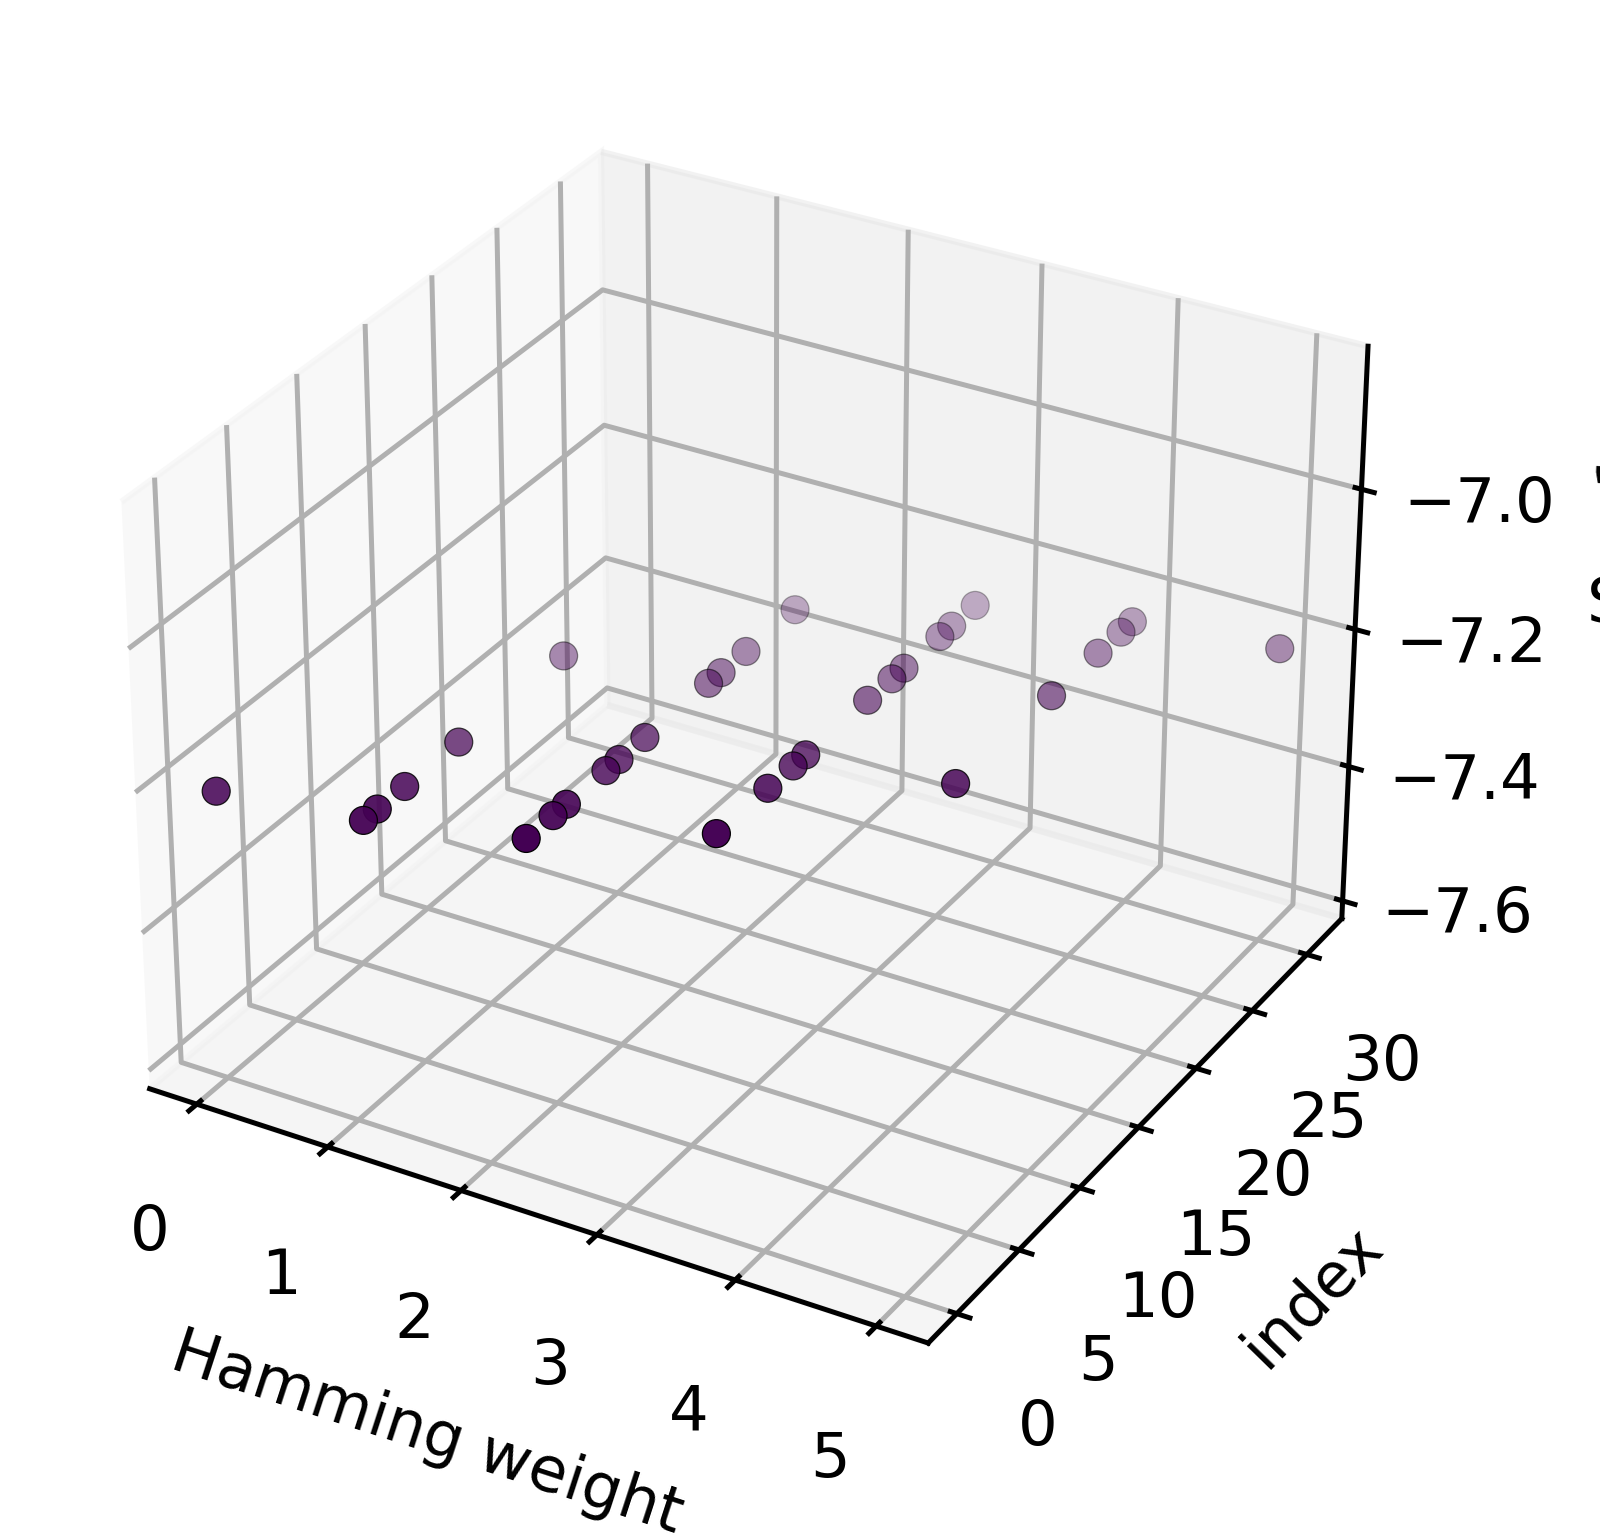
\includegraphics[width=\linewidth]{figs/branch_lattice.png}
  \caption{Phase-coloured branch lattice at depth
           $n=4$.  Opposite vertices differ by phase $\pi$ and interfere
           destructively when coarse-grained.}
  \label{fig:branch-lattice}
\end{figure}

\subsection{Emergent Schrödinger evolution}

Weight conservation and phase additivity imply a differential equation
in the continuum limit:

\[
  i\frac{\partial}{\partial n}\Psi_n
  =-\frac{\nabla^2}{2}\,\Psi_n + V\,\Psi_n + \order{n^{-1}},
\tag{4.5}\label{eq:schrod}
\]

where $V$ arises from ledger-tag curvature (explained in
Section~\ref{sec:gauge}).  Equation~\eqref{eq:schrod} is the discrete
Schrödinger equation, derived here from counting alone.

\subsection{Key points for later sections}

\begin{itemize}
  \item Born's rule (Theorem) removes the statistical postulate from
        quantum mechanics.
  \item Ledger phase explains interference without wavefunction
        "collapse"; branch pruning is merely coarse-graining.
  \item The discrete Laplacian in Eq.~\eqref{eq:schrod} will reappear
        as the curvature operator in Section~\ref{sec:mass}.
\end{itemize}

\clearpage
